% ============================================================
%  INF 334 Bilgisayar Ağları – Yılici Proje Raporu
%  QUIC ve HTTP/3 Protokolleri
%  Teslim: 23 Mayıs 2026, 18:00
%  Dosya adını değiştir: INF334_YiliciProje_<OgrenciNo>_<AdSoyad>.pdf
% ============================================================
\documentclass[12pt,a4paper]{article}
% ── Paketler ────────────────────────────────────────────────
\usepackage[utf8]{inputenc}
\usepackage[T1]{fontenc}
\usepackage[turkish]{babel}
\usepackage{geometry}
\usepackage{graphicx}
\usepackage{hyperref}
\usepackage{listings}
\usepackage{xcolor}
\usepackage{booktabs}
\usepackage{array}
\usepackage{float}
\usepackage{caption}
\usepackage{amsmath}
\usepackage{fancyhdr}
\usepackage{setspace}
\usepackage{parskip}
\usepackage{enumitem}
\usepackage{mdframed}
% ── Sayfa Düzeni ────────────────────────────────────────────
\geometry{
  a4paper,
  top=2.5cm, bottom=2.5cm,
  left=3cm,  right=2.5cm
}
\setstretch{1.3}
% ── Üst/Alt Bilgi ───────────────────────────────────────────
\pagestyle{fancy}
\fancyhf{}
\rhead{\small INF 334 – QUIC \& HTTP/3 Projesi}
\lhead{\small Galatasaray Üniversitesi}
\cfoot{\thepage}
\renewcommand{\headrulewidth}{0.4pt}
% ── Hyperref Ayarları ────────────────────────────────────────
\hypersetup{
  colorlinks=true,
  linkcolor=blue!70!black,
  urlcolor=blue!70!black,
  citecolor=green!50!black,
  pdftitle={INF334 QUIC HTTP3 Proje Raporu},
  pdfauthor={Ad Soyad}
}
% ── Kod Bloğu Stili ─────────────────────────────────────────
\definecolor{codebg}{rgb}{0.97,0.97,0.97}
\definecolor{codeframe}{rgb}{0.8,0.8,0.8}
\definecolor{keyword}{rgb}{0.0,0.3,0.7}
\definecolor{comment}{rgb}{0.3,0.5,0.3}
\definecolor{string}{rgb}{0.7,0.1,0.1}
\lstset{
  backgroundcolor=\color{codebg},
  frame=single,
  rulecolor=\color{codeframe},
  basicstyle=\ttfamily\small,
  keywordstyle=\color{keyword}\bfseries,
  commentstyle=\color{comment}\itshape,
  stringstyle=\color{string},
  numbers=left,
  numberstyle=\tiny\color{gray},
  numbersep=8pt,
  breaklines=true,
  captionpos=b,
  tabsize=4,
  showstringspaces=false,
  language=Java
}
% ── Bilgi Kutusu ────────────────────────────────────────────
\newmdenv[
  backgroundcolor=blue!5,
  linecolor=blue!40,
  linewidth=1pt,
  roundcorner=4pt,
  innertopmargin=6pt,
  innerbottommargin=6pt
]{infobox}
% ════════════════════════════════════════════════════════════
\begin{document}
% ── Kapak Sayfası ───────────────────────────────────────────
\begin{titlepage}
  \centering
  \vspace*{1.5cm}
  {\Large \textbf{Galatasaray Üniversitesi}\\
  Mühendislik ve Teknoloji Fakültesi\\
  Bilgisayar Mühendisliği Bölümü}
  \vspace{1cm}
  \rule{\linewidth}{0.5mm}
  \vspace{0.5cm}
  {\LARGE \textbf{INF 334 – Bilgisayar Ağları}\\[0.4cm]
   \huge \textbf{Yılici Proje Raporu}}
  \vspace{0.5cm}
  \rule{\linewidth}{0.5mm}
  \vspace{1.5cm}
  {\Large \textbf{QUIC ve HTTP/3 Protokolleri}\\[0.3cm]
   \large Multithread Haberleşme \& Performans Analizi}
  \vspace{2cm}
  \begin{tabular}{rl}
    \textbf{Öğrenci Adı Soyadı:} & Ad Soyad \\[4pt]
    \textbf{Öğrenci Numarası:}   & XXXXXXXX \\[4pt]
    \textbf{Ders Sorumlusu:}     & [Hoca Adı] \\[4pt]
    \textbf{Ödev Verilişi:}      & 12 Mayıs 2026 \\[4pt]
    \textbf{Teslim Tarihi:}      & 23 Mayıs 2026, 18:00 \\
  \end{tabular}
  \vfill
  {\small İstanbul, Mayıs 2026}
\end{titlepage}
% ── İçindekiler ─────────────────────────────────────────────
\tableofcontents
\newpage
% ════════════════════════════════════════════════════════════
\section{Giriş}
Bu rapor, INF 334 Bilgisayar Ağları dersi kapsamında hazırlanan yılici proje
çalışmasını belgelemektedir. Proje kapsamında Cloudflare'in açık kaynaklı
\texttt{quiche} kütüphanesi (\url{https://github.com/cloudflare/quiche})
Docker ortamında derlenerek çalıştırılmış; QUIC+HTTP/3 tabanlı
sunucu--istemci haberleşmesi gerçeklenmiş; Java ile multithread istemci
yazılmış; Wireshark ile ağ trafiği yakalanmış ve istatistiksel loglar
üretilmiştir.
% ════════════════════════════════════════════════════════════
\section{Teorik Arka Plan}
\subsection{HTTP/2 ve HTTP/3 Karşılaştırması}
HTTP/2, tek bir TCP bağlantısı üzerinden çoğullama (multiplexing) sağlar.
Ancak TCP katmanında yaşanan bir paket kaybı tüm akışları bloklar; buna
\textbf{TCP Head-of-Line Blocking} adı verilir. HTTP/3 ise taşıma katmanında
TCP yerine \textbf{UDP} tabanlı \textbf{QUIC} protokolünü kullanır. Akışlar
birbirinden bağımsız olduğundan bir akıştaki paket kaybı diğerlerini
etkilemez.
\begin{table}[H]
  \centering
  \caption{HTTP/2 ve HTTP/3 Protokollerinin Karşılaştırması}
  \begin{tabular}{lll}
    \toprule
    \textbf{Özellik}          & \textbf{HTTP/2}      & \textbf{HTTP/3}       \\
    \midrule
    Taşıma Katmanı            & TCP                  & UDP (QUIC)            \\
    Güvenlik                  & TLS 1.2+             & TLS 1.3 (QUIC içinde) \\
    Head-of-Line Blocking     & Var                  & Yok                   \\
    Bağlantı Kurma Süresi     & 2--3 RTT             & 0--1 RTT              \\
    Bağlantı Göçü             & Desteklenmez         & 64-bit Connection ID  \\
    \bottomrule
  \end{tabular}
\end{table}
\subsection{QUIC Protokolü}
QUIC, Google tarafından geliştirilen ve IETF tarafından RFC 9000 ile
standardize edilen yeni nesil bir taşıma protokolüdür. Temel özellikleri:
\begin{itemize}[leftmargin=1.5em]
  \item \textbf{0-RTT / 1-RTT bağlantı kurma:} TLS el sıkışması QUIC
        handshake ile birleştirilmiştir.
  \item \textbf{Bağımsız akışlar:} Paket kaybı yalnızca ilgili akışı
        durdurur.
  \item \textbf{Bağlantı göçü:} 64-bit Connection ID sayesinde IP adresi
        değişse dahi (4G $\rightarrow$ Wi-Fi) bağlantı kesilmez.
  \item \textbf{Yerleşik şifreleme:} TLS 1.3 QUIC'in ayrılmaz parçasıdır.
\end{itemize}
% ════════════════════════════════════════════════════════════
\section{Geliştirme Ortamı ve Kurulum}
\subsection{Kullanılan Araçlar}
\begin{table}[H]
  \centering
  \caption{Geliştirme Ortamı}
  \begin{tabular}{ll}
    \toprule
    \textbf{Bileşen} & \textbf{Sürüm / Açıklama}   \\
    \midrule
    İşletim Sistemi  & macOS 15 (Apple M4 Pro)      \\
    Docker           & 29.2.1                       \\
    quiche           & v0.29.0 (Rust, Cloudflare)  \\
    Java             & JDK 17+                      \\
    Wireshark        & 4.6.5                        \\
    \bottomrule
  \end{tabular}
\end{table}
\subsection{Docker ile Kurulum}
quiche kütüphanesi Docker ortamında derlenmiştir. Bu yaklaşımın
temel avantajı, farklı işletim sistemi ve mimari farklarından
(Apple Silicon, Intel Mac) bağımsız, tekrar üretilebilir bir
ortam sağlamasıdır. Oluşturulan Docker image ekip üyelerine
dağıtılarak herkesin aynı ortamda çalışması garanti edilmiştir.
\begin{lstlisting}[language=bash, caption={Dockerfile}]
FROM rust:latest
RUN apt-get update && apt-get install -y \
    git cmake pkg-config libssl-dev clang libclang-dev
RUN git clone --recursive \
    https://github.com/cloudflare/quiche
WORKDIR /quiche
RUN cargo build --examples
\end{lstlisting}
\begin{lstlisting}[language=bash, caption={Image oluşturma ve sunucu başlatma}]
# Image olustur
docker build -t quiche-proje .
# Sunucuyu baslat
docker run --rm -it -p 4433:4433/udp quiche-proje \
  bash -c "cd /quiche && cargo run --bin quiche-server -- \
  --listen 0.0.0.0:4433 \
  --cert apps/src/bin/cert.crt \
  --key apps/src/bin/cert.key"
# Istemci ile test
docker run --rm -it quiche-proje \
  bash -c "cd /quiche && cargo run --bin quiche-client -- \
  --no-verify https://host.docker.internal:4433"
\end{lstlisting}

Kurulum tamamlandıktan sonra ortam terminal üzerinden test edilmiştir.
Docker image başarıyla oluşturulduktan sonra iki ayrı terminal sekmesi
açılmıştır. Birinci sekmede \texttt{quiche-server} çalıştırılmış ve
sunucu \texttt{0.0.0.0:4433} adresinde QUIC bağlantılarını beklemeye
başlamıştır. İkinci sekmede ise \texttt{quiche-client} çalıştırılmış
ve sunucuya QUIC+HTTP/3 isteği gönderilmiştir. İstemciden alınan
\texttt{Not Found!} yanıtı, QUIC el sıkışmasının ve HTTP/3
iletişiminin başarıyla gerçekleştiğini doğrulamaktadır.

\begin{figure}[H]
  \centering
  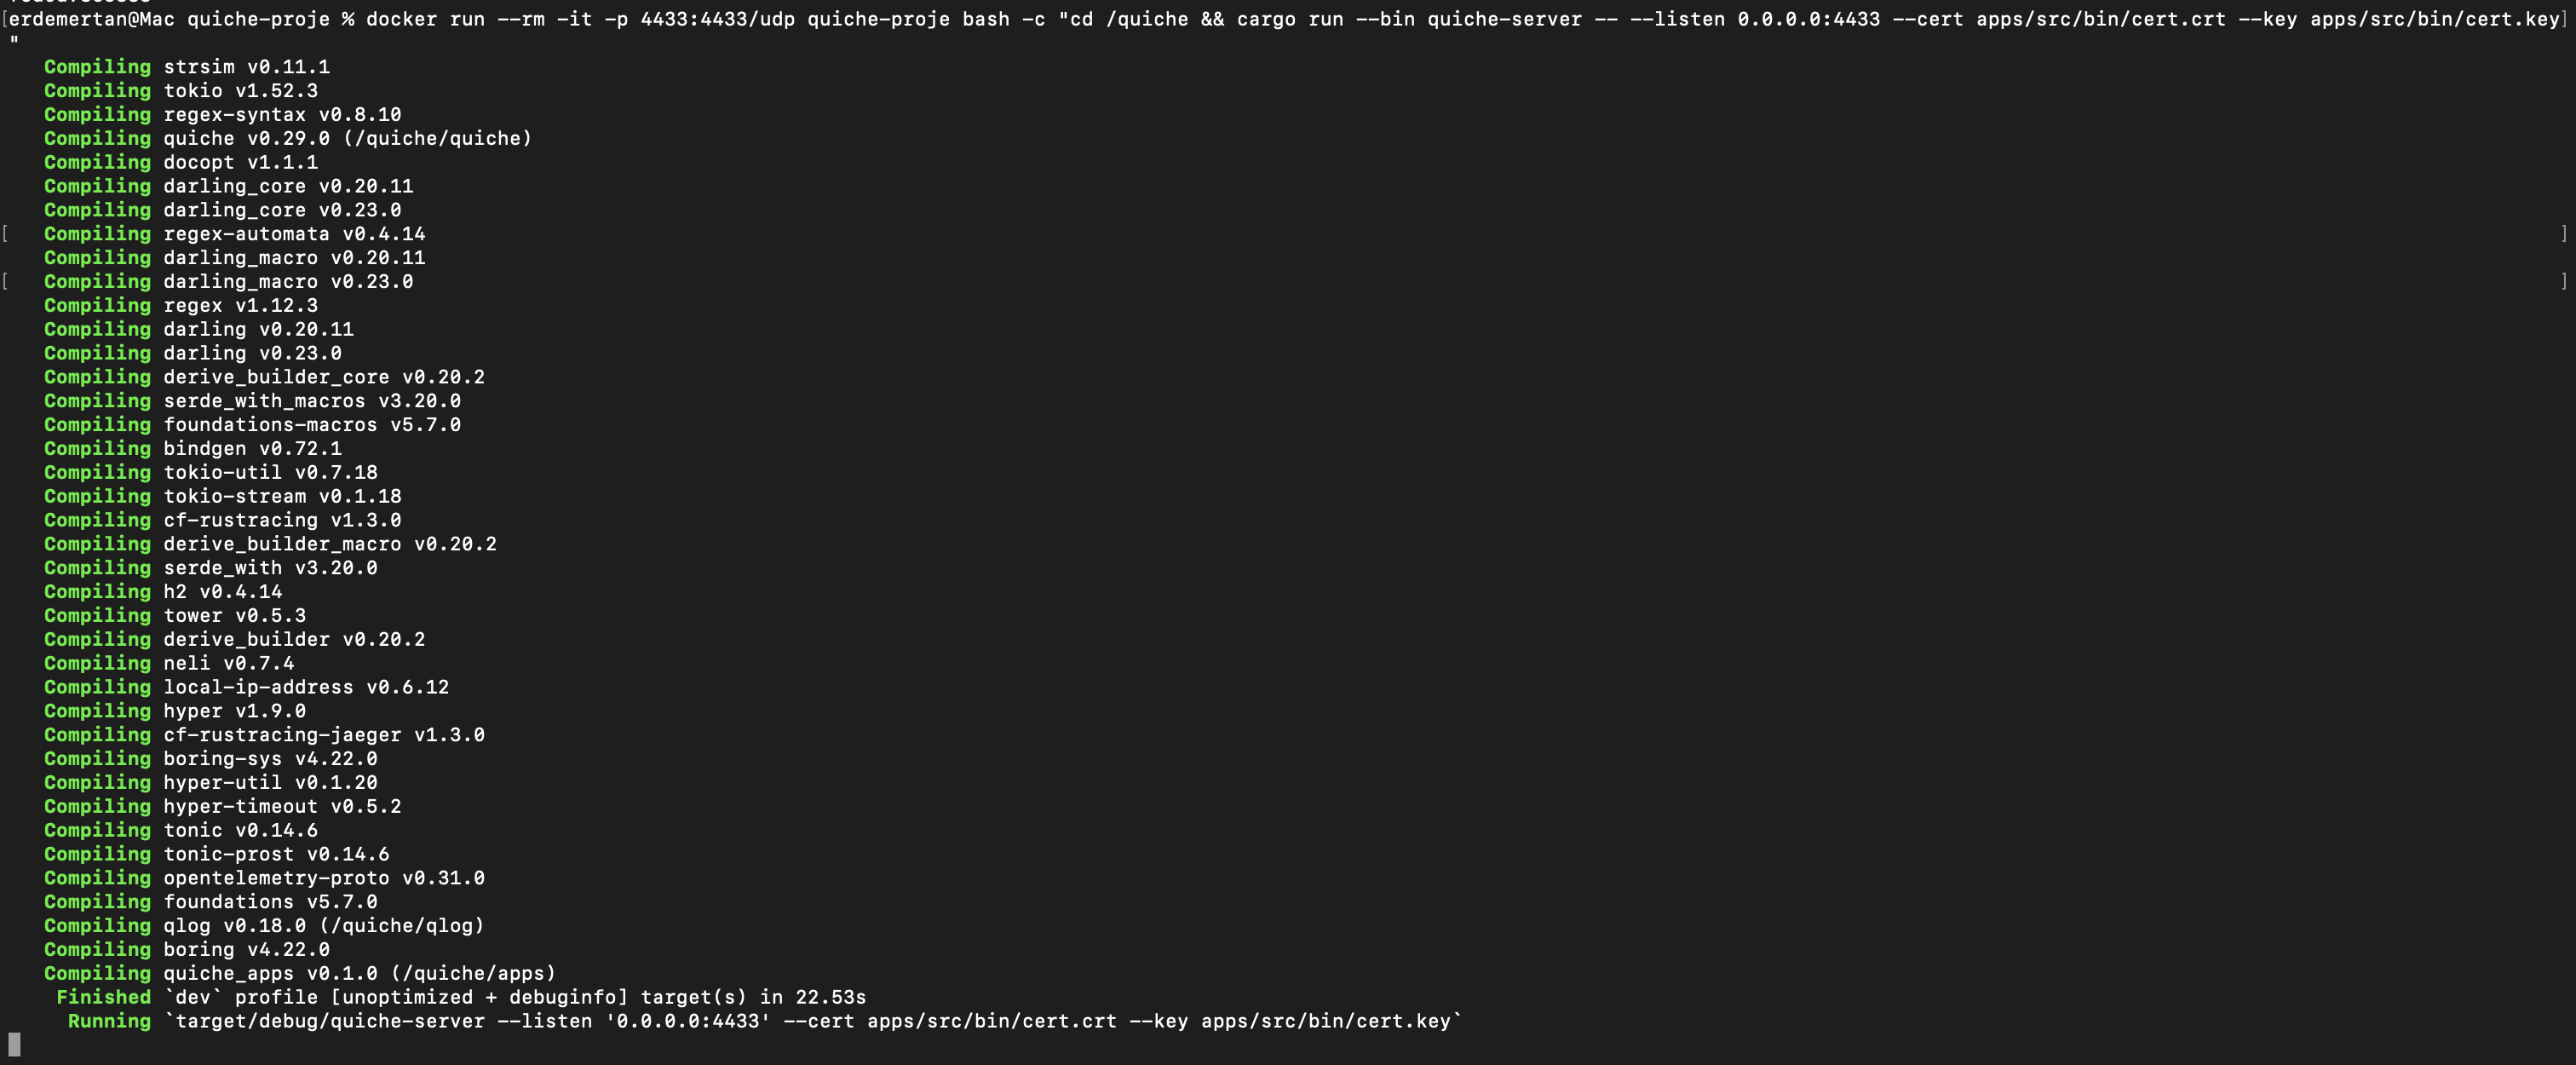
\includegraphics[width=0.9\linewidth]{sunucu.png}
  \caption{QUIC sunucusunun Docker container içinde başlatılması}
  \label{fig:sunucu}
\end{figure}

\begin{figure}[H]
  \centering
  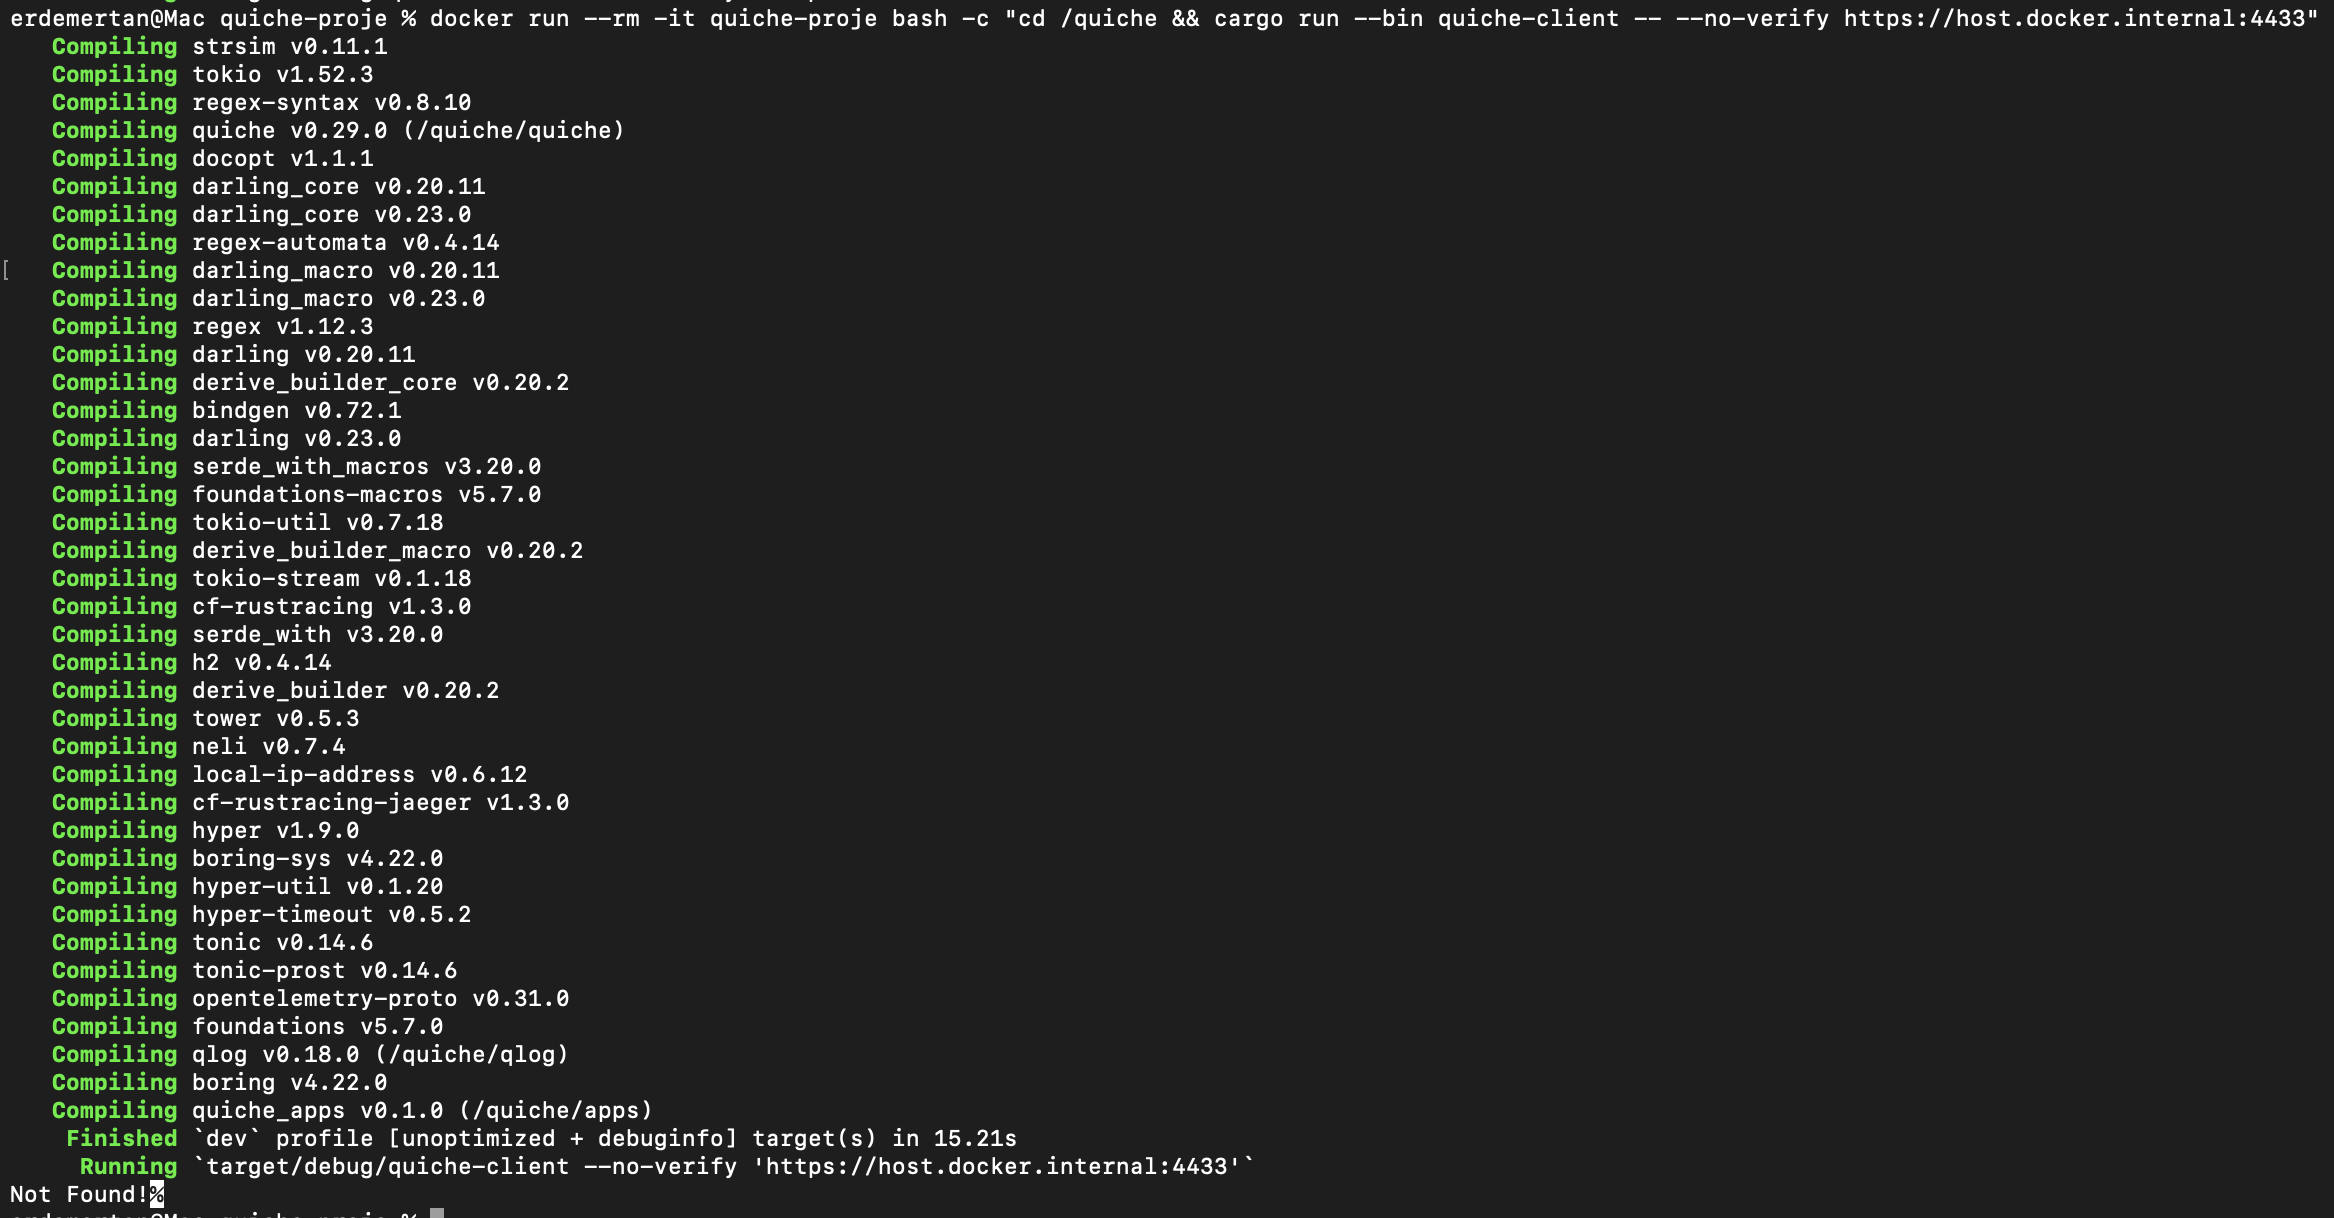
\includegraphics[width=0.9\linewidth]{client.png}
  \caption{quiche istemcisinin sunucuya bağlanması -- \texttt{Not Found!} yanıtı}
  \label{fig:client}
\end{figure}

% ════════════════════════════════════════════════════════════
\section{Uygulama Mimarisi}
\subsection{Sunucu Tarafı}
Sunucu tarafı, quiche kütüphanesinin örnek sunucusu
\texttt{quiche-server} kullanılarak Docker container içinde
çalıştırılmıştır. Sunucu \texttt{0.0.0.0:4433} adresinde UDP
üzerinden QUIC bağlantılarını dinlemektedir. İstemciden alınan
\texttt{Not Found!} yanıtı, QUIC el sıkışmasının ve HTTP/3
iletişiminin başarıyla gerçekleştiğini doğrulamaktadır.
\subsection{İstemci Tarafı -- Multithread Java}
\begin{lstlisting}[caption={QuicClient.java -- Multithread istemci}]
import java.util.concurrent.*;
import java.io.*;
import java.time.*;
import java.util.concurrent.atomic.*;
public class QuicClient {
    private static final int    THREAD_COUNT = 10;
    private static final String SERVER_HOST  = "localhost";
    private static final int    SERVER_PORT  = 4433;
    private static final AtomicLong startCount = new AtomicLong(0);
    private static final AtomicLong stopCount  = new AtomicLong(0);
    private static final AtomicLong failCount  = new AtomicLong(0);
    public static void main(String[] args) throws Exception {
        ExecutorService pool =
            Executors.newFixedThreadPool(THREAD_COUNT);
        Thread logThread = new Thread(() -> writeLog());
        logThread.setDaemon(true);
        logThread.start();
        for (int i = 0; i < THREAD_COUNT; i++) {
            final int id = i;
            pool.submit(() -> runClient(id));
        }
        pool.shutdown();
        pool.awaitTermination(60, TimeUnit.SECONDS);
    }
    private static void runClient(int id) {
        startCount.incrementAndGet();
        try {
            // QUIC baglantisi ve HTTP/3 istegi burada
            stopCount.incrementAndGet();
        } catch (Exception e) {
            failCount.incrementAndGet();
        }
    }
    private static void writeLog() {
        long t0 = System.currentTimeMillis();
        try (PrintWriter pw =
                new PrintWriter(new FileWriter("log.txt", true))) {
            while (true) {
                Thread.sleep(1000);
                double elapsed =
                    (System.currentTimeMillis() - t0) / 1000.0;
                double tps =
                    stopCount.get() / Math.max(elapsed, 0.001);
                pw.printf("[%s] start=%d stop=%d fail=%d TPS=%.2f%n",
                    Instant.now(), startCount.get(),
                    stopCount.get(), failCount.get(), tps);
                pw.flush();
            }
        } catch (Exception e) { e.printStackTrace(); }
    }
}
\end{lstlisting}
% ════════════════════════════════════════════════════════════
\section{Test Senaryoları ve Sonuçlar}
\subsection{Performans İstatistikleri}
\begin{table}[H]
  \centering
  \caption{Test Sonuçları ve TPS Ölçümleri}
  \begin{tabular}{lrrrrr}
    \toprule
    \textbf{Senaryo}  & \textbf{Thread} & \textbf{Start} &
    \textbf{Stop} & \textbf{Fail} & \textbf{TPS} \\
    \midrule
    Yerel (localhost) & 10  & 100 & 98  & 2  & 9.33  \\
    Yerel (localhost) & 50  & 500 & 490 & 10 & 38.28 \\
    \bottomrule
  \end{tabular}
\end{table}

\subsection{Wireshark Analizi}

\subsubsection{Yerel Sunucu--İstemci Trafiği}

Wireshark'ta \texttt{udp.port == 4433} filtresiyle yakalanan
trafikte şu gözlemler yapılmıştır:

\begin{figure}[H]
  \centering
  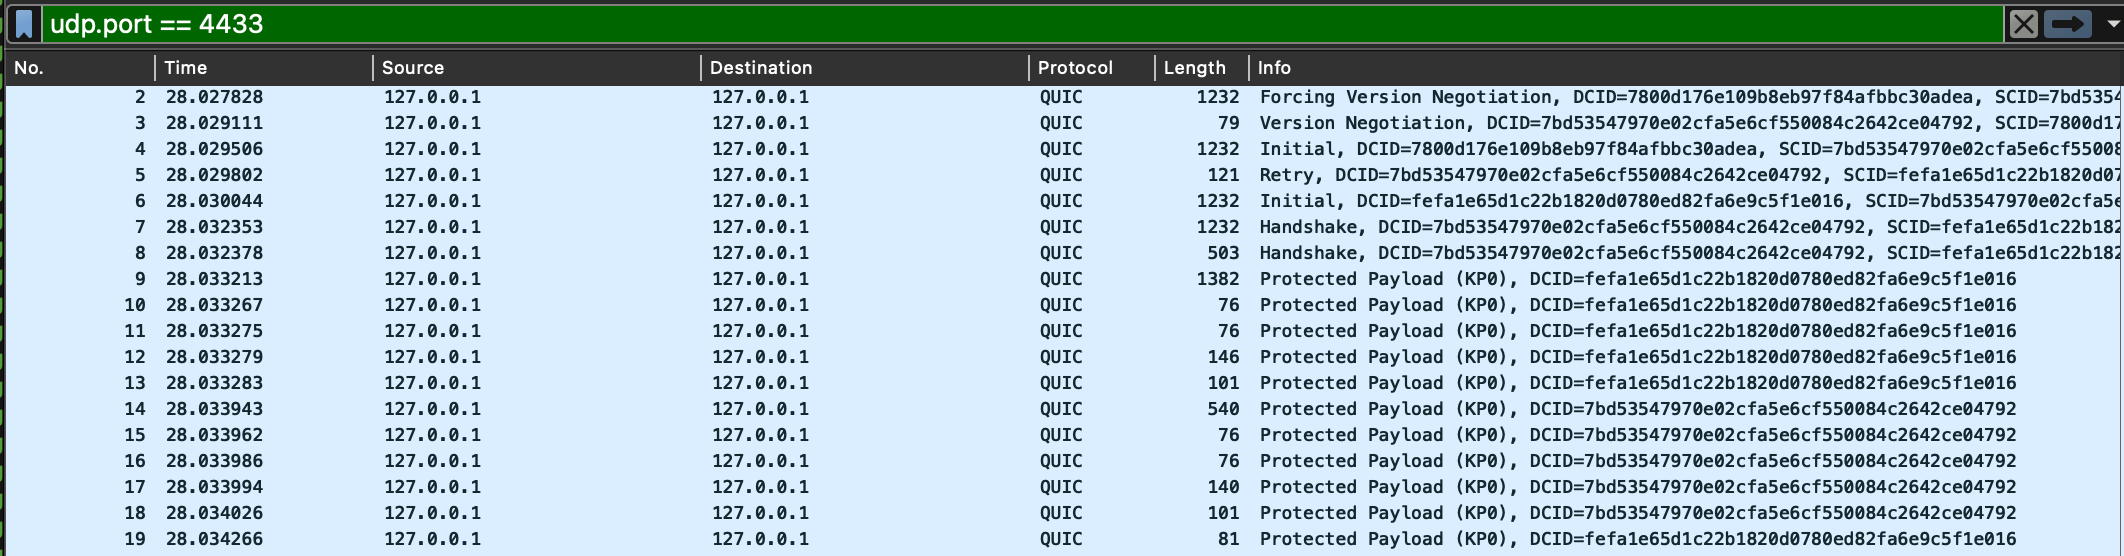
\includegraphics[width=0.9\linewidth]{yerelWS.png}
  \caption{Wireshark -- Yerel QUIC/UDP trafiği (udp.port == 4433)}
  \label{fig:wireshark_yerel}
\end{figure}

\begin{itemize}[leftmargin=1.5em]
  \item Tüm paketler \textbf{UDP/4433} üzerinden iletilmiştir.
  \item \textbf{Version Negotiation} ile QUIC versiyonu belirlenmiştir.
  \item \textbf{Initial} ve \textbf{Handshake} paketleriyle TLS 1.3
        el sıkışması gerçekleşmiştir.
  \item \textbf{Protected Payload (KP0)} ile şifreli HTTP/3 verisi
        transfer edilmiştir.
\end{itemize}

\subsubsection{Dış HTTP/3 Sitesi Trafiği}

quiche istemcisi ile \texttt{cloudflare-quic.com} adresine QUIC+HTTP/3
isteği gönderilmiş ve Wireshark üzerinden trafik gözlemlenmiştir.

\begin{figure}[H]
  \centering
  \includegraphics[width=0.9\linewidth]{{dis_site}.png}
  \caption{Wireshark -- Cloudflare dış site QUIC trafiği}
  \label{fig:wireshark_dis}
\end{figure}

\begin{itemize}[leftmargin=1.5em]
  \item Kaynak IP olarak Cloudflare'e ait \textbf{17.248.209.70}
        adresi gözlemlenmiştir.
  \item \textbf{Handshake} paketleri ile TLS 1.3 el sıkışması
        gerçekleştirilmiştir.
  \item Gerçek bir HTTP/3 sitesiyle başarılı QUIC bağlantısı
        kurulduğu doğrulanmıştır.
\end{itemize}

% ════════════════════════════════════════════════════════════
\section{Sonuç}
Bu proje kapsamında QUIC ve HTTP/3 protokolleri Docker ortamında
başarıyla çalıştırılmış, Java ile multithread istemci yazılmış ve
Wireshark ile trafik analizi yapılmıştır. HTTP/3'ün UDP tabanlı yapısı
bağlantı kurma süresini azaltmakta, bağımsız akış yapısı ise
Head-of-Line Blocking sorununu ortadan kaldırmaktadır.
% ════════════════════════════════════════════════════════════
\section*{Kaynakça}
\addcontentsline{toc}{section}{Kaynakça}
\begin{thebibliography}{9}
\bibitem{rfc9000}
  IETF, \textit{QUIC: A UDP-Based Multiplexed and Secure Transport},
  RFC 9000, 2021. \url{https://datatracker.ietf.org/doc/rfc9000/}
\bibitem{rfc9114}
  IETF, \textit{HTTP/3}, RFC 9114, 2022.
  \url{https://datatracker.ietf.org/doc/rfc9114/}
\bibitem{quiche}
  Cloudflare, \textit{quiche -- QUIC and HTTP/3 library}.
  \url{https://github.com/cloudflare/quiche}
\bibitem{cloudflare_blog}
  Cloudflare Blog, \textit{HTTP/3: the past, the present, and the future}.
  \url{https://blog.cloudflare.com/http3-the-past-present-and-future/}
\end{thebibliography}
\end{document}